\subsubsubsubsection{Stop}
\begin{figure}[h]
\centering
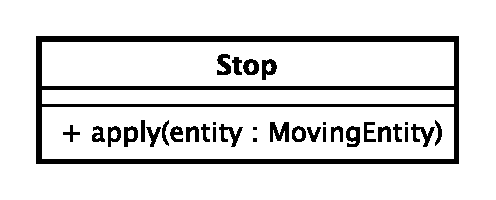
\includegraphics[scale=0.6,keepaspectratio]{images/solution/app/backend/stop.eps}
\caption{\pPassive::Stop}
\label{fig:sd-app-stop}
\end{figure}
\FloatBarrier
\begin{itemize}
  \item \textbf{\descr} \\
It implements the stop road sign. It registers the traveller for a timeout.
  \item \textbf{\ops}
  \begin{itemize} 
  \item[+] \texttt{apply(pedestrian: Pedestrian)} \\
Registers the pedestrian for a timeout.
  \item[+] \texttt{apply(vehicle: Vehicle)} \\
Registers the vehicle for a timeout.
  \end{itemize}
\end{itemize}
